\subsection{All to finish application}
    We can extend the previous application to an all-to-finish operator, this operator can for instance parallel work, a task that requires a lot of computation and can be done in separate pieces by separate workers. \cite{dq-tut}

        \subsubsection{Introducing a slower component}
            Like we did for the FTF operator, let's introduce a slower work into the mix. We introduce a slight delay to show how even a few milliseconds can be noticeable right away by a keen eye (or by triggers, which avoids having to look constantly at the graphs). The delay is a 2ms sleep on worker\_2.
 
            The difference in the worker's $\Delta$Q can be noticed with $\Delta \text{Q}_{w2} > \Delta \text{Q}_{w1}$. The difference can then be observed in the all-to-finish plot, where the operator's $\Delta$Qs (both observed and calculated) can be overlaid on top of worker\_2 $\Delta$Q, showing once again that the $\Delta$QSD algebraic foundation is sound.

            \begin{figure}[H]
                \begin{center}
                    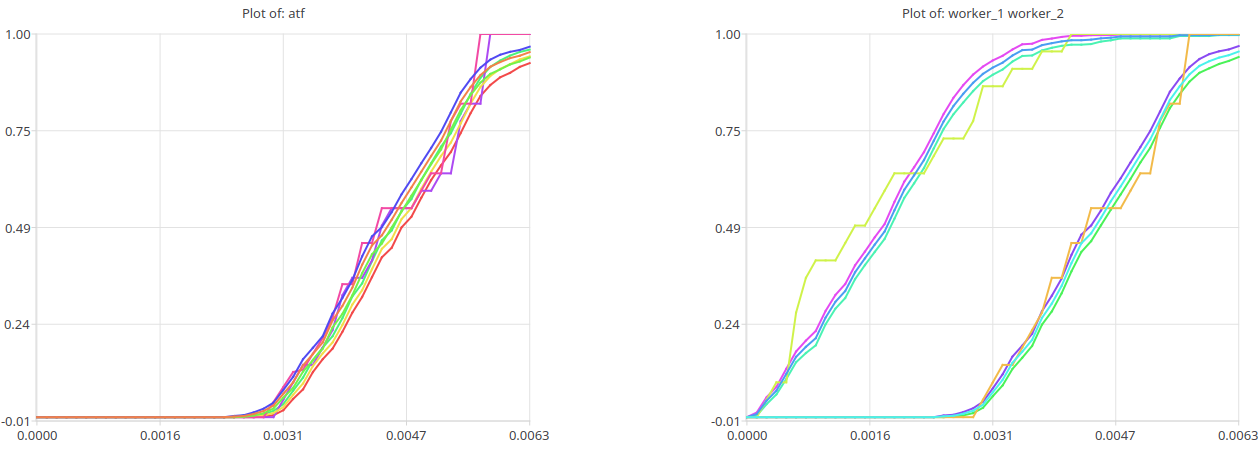
\includegraphics[scale = 0.5]{img/overload_2/w1w2atf.png}
                \end{center}
            \end{figure}

    These plots show the usefulness of $\Delta$QSD, the system can be decomposed to understand which part of the system is showing hazards, furthermore, the causal relationships can be observed to determine the behaviour of a part down to the single component.
